\documentclass[12pt,a4paper]{article}
\usepackage{graphicx}
\usepackage{geometry}
\usepackage{setspace}
\usepackage{enumitem}      
\usepackage[table]{xcolor} 
\usepackage{array}         

\definecolor{kublue}{RGB}{0, 85, 164}       
\definecolor{lightblue}{RGB}{235, 243, 250} 

\geometry{margin=1in}
\setstretch{1.5}

\begin{document}

\begin{center}

\textbf{\large Kathmandu University}\\
\textbf{Department of Computer Science and Engineering}\\
\textbf{Dhulikhel, Kavrepalanchowk}

\vspace{0.8cm}


\includegraphics[width=4cm]{image/ku_logo.png}

\vspace{0.8cm}

\textbf{A Lab Report}\\
\textbf{On}\\
\textbf{``Compiler Design''}\\
\vspace{0.3cm}
\textbf{Lab Report: 2}\\
\textbf{[Code No: COMP 409]}

\vspace{1cm}

\textbf{Submitted by:}\\
Name: Prabin Aryal\\
Group: CE IV/I\\
Roll No: 08

\vspace{1cm}

\textbf{Submitted to:}\\
Mr. Sushil Nepal\\
Department of Computer Science and Engineering

\vspace{1cm}

\textbf{Submission Date:} 2026/06/12

\end{center}

\newpage

\section*{Aim}
To implement a regular expression and verify whether the input string is valid or invalid.

\section*{Theory}
A regular expression is a formal way to describe a set of strings. It helps us to represent patterns of strings.
Here, we are checking for the regular expression:

(a ( b + a )* b) + (b ( a + b ) * a)

Where,\\
a, b = input characters\\
e = epsilon (null)\\
+ = union\\
* = closure

This helps us to combine pattern matching, alphabet validation and structural property checking.

\section*{Algorithm}
\begin{enumerate}[label=\arabic*.]
    \item Input a string
    \item Compute the length of string
    \item If character is not a, b and e, declare INVALID string
    \item Elseif character is e, taken as NULL and declare INVALID.
    \item If length $<$ 2, declare INVALID.
    \item Identify first and last character,
    \begin{enumerate}[label=\alph*.]
        \item if (first = a AND last = b) OR (first = b AND last = a), declare VALID.
        \item Else, declare INVALID
    \end{enumerate}
    \item Terminate
\end{enumerate}

\section*{Working}
\begin{figure}[h]
    \centering
    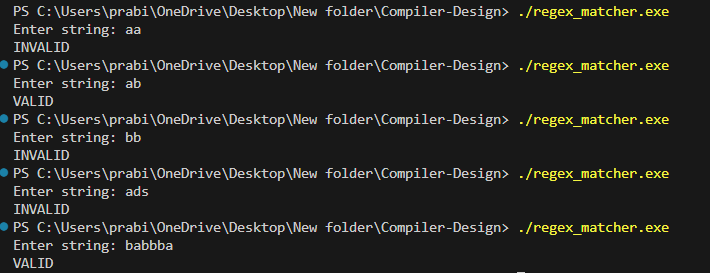
\includegraphics[width=0.8\textwidth]{image/regex_matcher.png}
    \caption{Output}
\end{figure}

\section*{Result}
In the end, we were successfully able to recognize the validity of the strings according to the taken regular expression.

\section*{Code}
The github link to code file: \texttt{https://github.com/vibingprabin/Compiler-Design.git}

\end{document}
